\documentclass[12pt, a4paper, bibliography=totoc]{scrarticle}


\usepackage[utf8]{inputenc}
\usepackage[T1]{fontenc}
\usepackage[english]{babel}
\usepackage[margin=2cm]{geometry}
\usepackage{placeins}

\usepackage{graphicx}
\usepackage{booktabs}
\usepackage{authblk}

\usepackage{tikz}
\usetikzlibrary{positioning, arrows.meta, calc}

\usepackage{pdflscape}

\usepackage{lipsum}

\usepackage{xcolor}
\usepackage[
colorlinks=true,
linkcolor=blue!70!black,
citecolor=blue!70!black,
urlcolor=blue!70!black
]{hyperref}


\usepackage[
backend=biber,
style=numeric,
sorting=none
]{biblatex}

\addbibresource{references.bib}

\usepackage[nameinlink, capitalize]{cleveref}
\usepackage{siunitx}
\sisetup{detect-all}
\sisetup{per-mode = symbol-or-fraction}
\DeclareSIUnit{\revpermin}{rpm}
\DeclareSIUnit{\inch}{in}


% Title Page
\title{Pitch Angle Correction for DIC Measurements}
\author{José A. Rosas Córdova}
\author{Jasson Printezis}

\affil[]{Institut für Turbomaschinen und Fluid-Dynamik}

\begin{document}
	\maketitle
	
	
	\tableofcontents
	\clearpage
	
	\section{Introduction}
	The measurement of aeroelastic deformations on wind turbines based on digital image correlation has been an ongoing project at the TFD with gradual contributions being made on different areas of the project through the years \cite{gossling2020qualifizierung,steimer2026auswertung,lehnhoff2026validation,winstroth2020optische}. 
	
	One of the current focuses of the project is to allow for processing longer datasets to capture a longer operating window of the turbine rotor. While different methodologies have been employed to ameliorate the data load in the processing pipeline \cite{automatisierung_auswertung_dic_2025}, not enough had been done to accommodate changes in the operational state of the wind turbine as a product of the ever changing wind conditions at the measurement site. 
	
	The subsequent text illustrates two correction processes implemented into the current transformation script to counteract the effects of changes in the wind turbine yaw angle as well as the individual pitching of the blades. The procedures were qualitatively tested with a real world dataset (i.e. \textit{Messung24}) as well as bench-marked against a synthetic measurement generated using a Blender model of a wind turbine and known deformation values.
	
	\section{Yaw Correction}
	\subsection{Problem Statement}
	As the length of the measurements increases, changes in the orientation of the wind turbine as a product of wind direction changes become increasingly common. The present operation sequence followed by the \textit{align\_coordinate\_systems.py} script is shown in \cref{fig:original_pipeline}. Since the process currently only considers the rotation matrix computed using the averaged circle to transform all the frames, the resulting transformed coordinates are bound to accumulate a certain amount of error, specially if the rotor orientation in the frame they belong to does not agree well with the averaged circle used to compute the transformations (e.g. when the wind turbine changes its yaw angle during the recording).
	\begin{figure}[htbp]
		\centering
		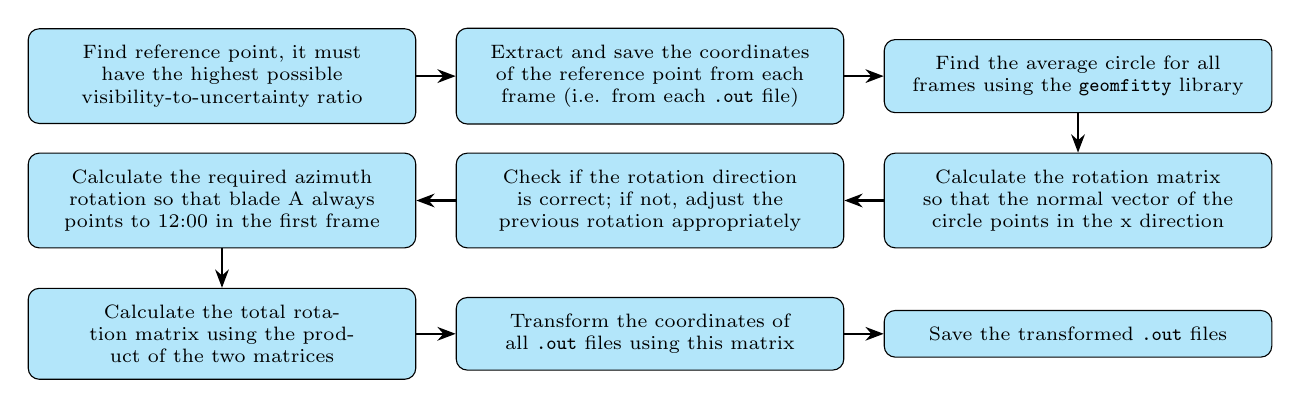
\begin{tikzpicture}[
			node distance = 0.5cm and 0.5cm,
			mybox/.style = {
				rectangle,
				rounded corners,
				draw=black,
				fill=cyan!30,
				text width=4.5cm,
				align=center,
				minimum height=0.5cm,
				font=\scriptsize,
				inner sep=6pt
			},
			line/.style = {-{Stealth}, thick}
			]
			% Row 1 (Left to Right)
			\node[mybox] (p1) {Find reference point, it must have the highest possible visibility-to-uncertainty ratio};
			\node[mybox, right=of p1] (p2) {Extract and save the coordinates of the reference point from each frame (i.e. from each \texttt{.out} file)};
			\node[mybox, right=of p2] (p3) {Find the average circle for all frames using the \texttt{geomfitty} library};
			
			% Row 2 (Right to Left)
			\node[mybox, below= of p3] (p4) {Calculate the rotation matrix so that the normal vector of the circle points in the x direction};
			\node[mybox, left=of p4] (p5) {Check if the rotation direction is correct; if not, adjust the previous rotation appropriately};
			\node[mybox, left=of p5] (p6) {Calculate the required azimuth rotation so that blade A always points to 12:00 in the first frame};
			
			% Row 3 (Left to Right)
			\node[mybox, below= of p6] (p7) {Calculate the total rotation matrix using the product of the two matrices};
			\node[mybox, right=of p7] (p8) {Transform the coordinates of all \texttt{.out} files using this matrix};
			\node[mybox, right=of p8] (p9) {Save the transformed \texttt{.out} files};
			
			% Arrows - Row 1
			\draw[line] (p1) -- (p2);
			\draw[line] (p2) -- (p3);
			
			% Transition from Row 1 to Row 2
			\draw[line] (p3) -- (p4);
			
			% Arrows - Row 2
			\draw[line] (p4) -- (p5);
			\draw[line] (p5) -- (p6);
			
			% Transition from Row 2 to Row 3
			\draw[line] (p6) -- (p7);
			
			% Arrows - Row 3
			\draw[line] (p7) -- (p8);
			\draw[line] (p8) -- (p9);
			
		\end{tikzpicture}
		\caption{Flow diagram of the transformations carried out within the original \textit{align\_coordinate\_system.py} script as described in \cite{automatisierung_auswertung_dic_2025}.}
		\label{fig:original_pipeline}
	\end{figure}
	
	An undesired result of this simplified alignment process is a clear divergence of the calculated blade torsion values whenever a change in the turbine yaw angle is present. A clear example of this effect can be seen in \cref{fig:yaw_problem_statement}.
	\begin{figure}[h]
		\centering
		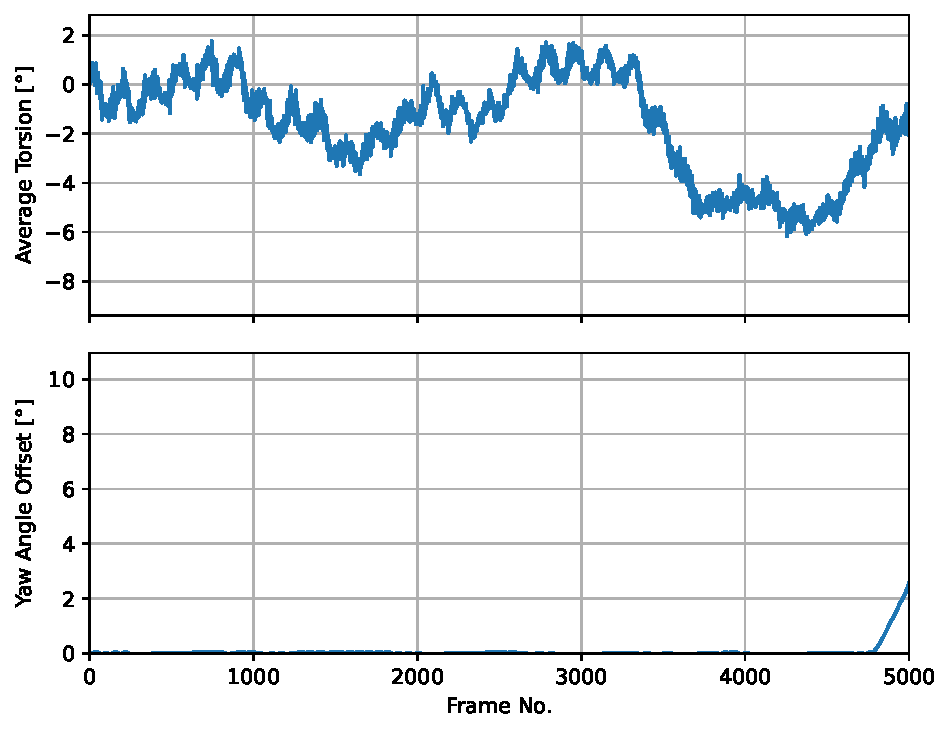
\includegraphics[width=0.6\linewidth]{graphics/yaw_problem_statement.pdf}
		\caption{Averaged measured torsion of the third AoI of blade A recorded in the \textit{Messung 24} measurement plotted on top of the yaw angle offset.}
		\label{fig:yaw_problem_statement}
	\end{figure}
	
	\subsection{Solution Approach}
	\Cref{fig:new_ablauf} shows a flow diagram representation of the updated transformation sequence. Instead of using a circle averaged over the whole recording to carry out the linear transformation of all frames, an individual circle is fitted for each frame to approximate the current rotor orientation; this is then used to compute a frame-specific rotation matrix that is then used to transform the \textit{.out} file into the new coordinate system, aligning the axis of the rotor with the global x-axis for each frame.
	\begin{figure}[ht]
		\centering
		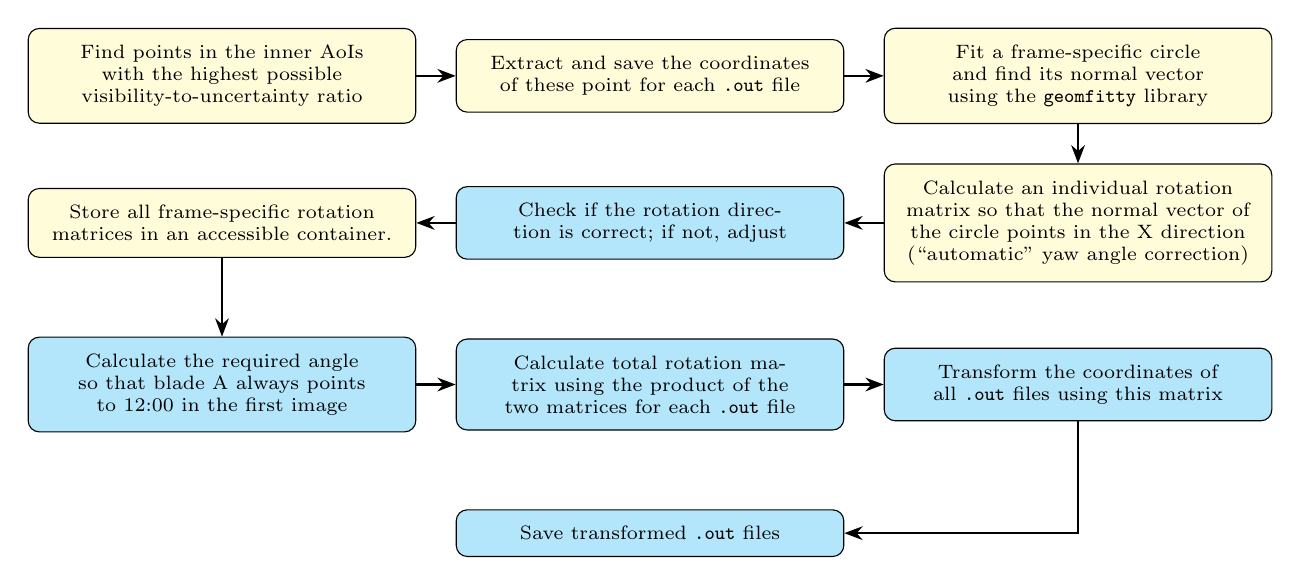
\begin{tikzpicture}[
			node distance = 0.5cm and 0.5cm,
			bluebox/.style = {
				rectangle,
				rounded corners,
				draw=black,
				fill=cyan!30,
				text width=4.5cm,
				align=center,
				minimum height=0.5cm,
				font=\scriptsize,
				inner sep=6pt
			},
			yellowbox/.style = {
				rectangle,
				draw=black,
				rounded corners,
				fill=yellow!15,
				text width=4.5cm,
				align=center,
				minimum height=0.5cm,
				font=\scriptsize,
				inner sep=6pt
			},
			line/.style = {-{Stealth}, thick}
			]
			% --- Row 1 (Left to Right) ---
			\node[yellowbox] (p1) {Find points in the inner AoIs with the highest possible visibility-to-uncertainty ratio};
			\node[yellowbox, right=of p1] (p2) {Extract and save the coordinates of these point for each \texttt{.out} file};
			\node[yellowbox, right=of p2] (p3) {Fit a frame-specific circle and find its normal vector using the \texttt{geomfitty} library};
			
			% --- Row 2 (Right to Left) ---
			\node[yellowbox, below= of p3] (p4) {Calculate an individual rotation matrix so that the normal vector of the circle points in the X direction (``automatic'' yaw angle correction)};
			\node[bluebox, left=of p4] (p5) {Check if the rotation direction is correct; if not, adjust};
			\node[yellowbox, left=of p5] (p6) {Store all frame-specific rotation matrices in an accessible container.};
			
			% --- Row 3 (Left to Right) ---
			\node[bluebox, below=1cm of p6] (p7) {Calculate the required angle so that blade A always points to 12:00 in the first image};
			\node[bluebox, right=of p7] (p8) {Calculate total rotation matrix using the product of the two matrices for each \texttt{.out} file};
			\node[bluebox, right=of p8] (p9) {Transform the coordinates of all \texttt{.out} files using this matrix};
			
			% --- Row 4 (Bottom Center/Right Flow) ---
			\node[bluebox, below=1.0cm of p8] (p10) {Save transformed \texttt{.out} files};
			
			% --- Connectors ---
			% Row 1
			\draw[line] (p1) -- (p2);
			\draw[line] (p2) -- (p3);
			
			% Row 1 -> Row 2
			\draw[line] (p3) -- (p4);
			
			% Row 2
			\draw[line] (p4) -- (p5);
			\draw[line] (p5) -- (p6);
			
			% Row 2 -> Row 3
			\draw[line] (p6) -- (p7);
			
			% Row 3
			\draw[line] (p7) -- (p8);
			\draw[line] (p8) -- (p9);
			
			% Row 3 -> Row 4
			\draw[line] (p9.south) |- (p10.east);
			
		\end{tikzpicture}
		\caption{Updated flow diagram of the transformations carried out within the \textit{align\_coordinate\_system.py}. The blocks in yellow show how the new computations fit within the old transformation sequence.}
		\label{fig:new_ablauf}
	\end{figure}
	
	
	\subsection{Results and Validation}
	During the development of the correction procedure the previously shown \textit{Messung24} dataset was used as a benchmark. A direct comparison of the resulting averaged torsion values with and without correction can be seen in \cref{fig:yaw_messung24}. When compared to the original signal, it is pretty evident how the amplitude of the orange line, corresponding to the corrected values, has been decoupled from the changes in the rotor yaw.
	\begin{figure}[h]
		\centering
		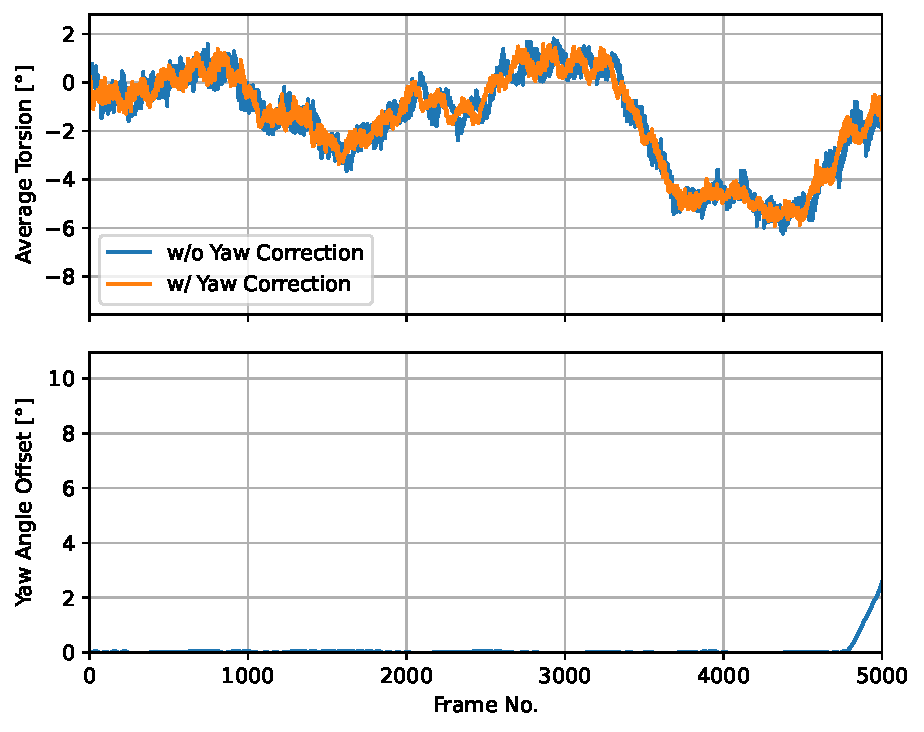
\includegraphics[width=0.6\linewidth]{graphics/yaw_messung24.pdf}
		\caption{Average torsion time-series for the third AoI in blade A with and without yaw correction.}
		\label{fig:yaw_messung24}
	\end{figure}
	
	
	Although these preliminary results looked qualitatively promising, since the dataset used during the development of the script emanated from a real-world measurement it was not possible to quantitatively evaluate how good the corrected results were with respect to a known baseline. With this in mind, a digital twin in the form of a Blender model was used as a known baseline to evaluate the obtained results against. 
	
	The outer section of the blender model blades were configured to follow a predefined torsion signal. The frames were generated and processed using the pipeline shown in Appendix \ref{appendix:a} and the corrected results finally compared with the known baseline. The resulting averaged torsion curves can be seen in \cref{fig:yaw_blender}
	\begin{figure}[h]
		\centering
		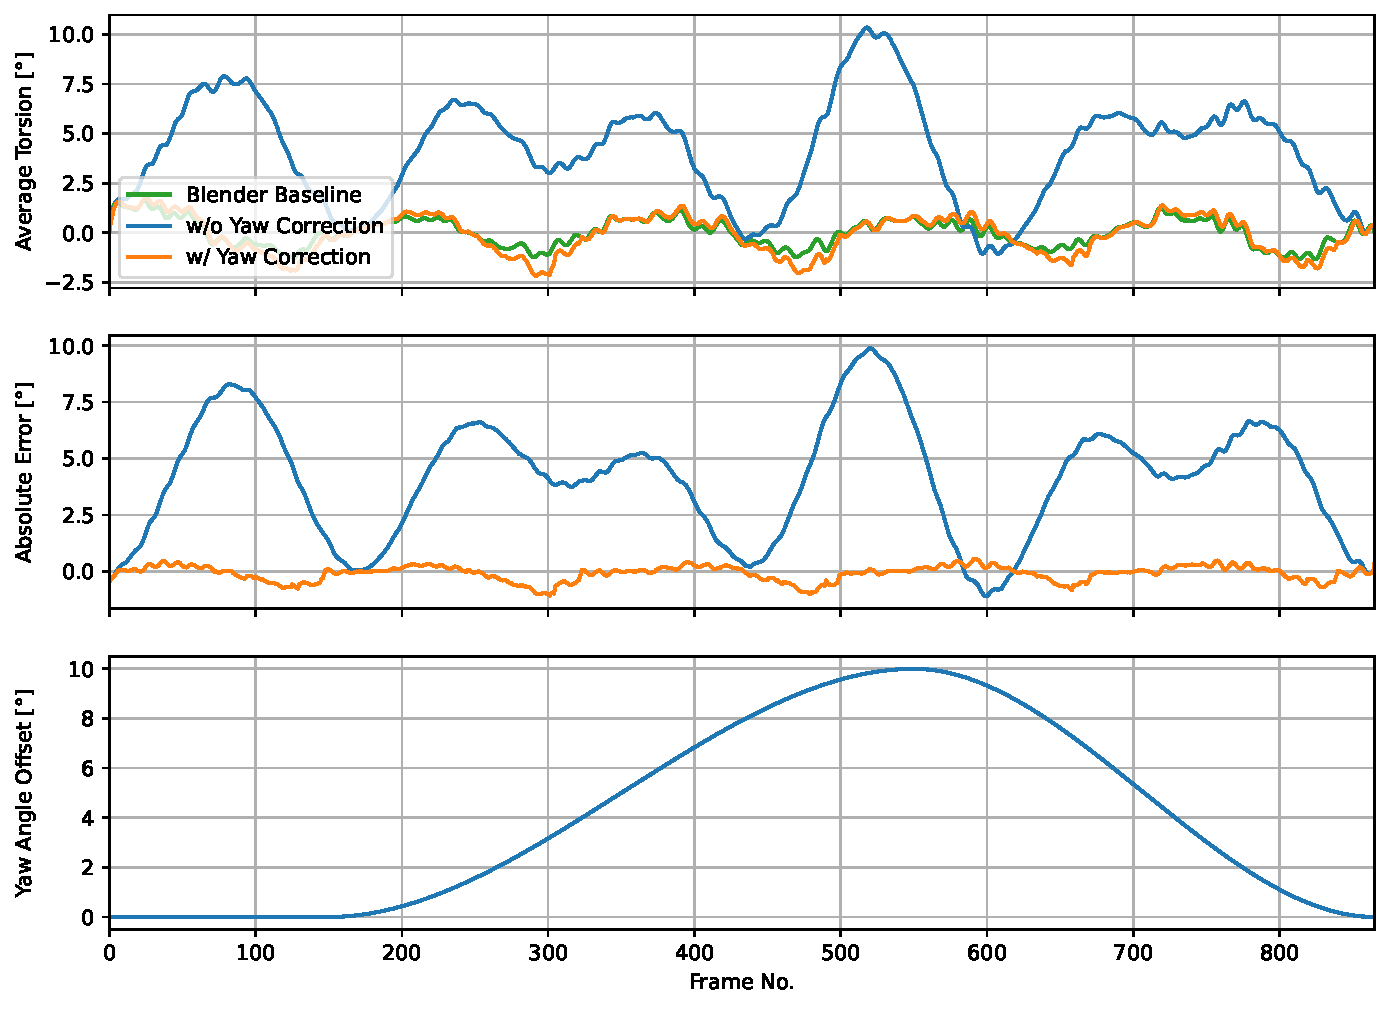
\includegraphics[width=0.6\linewidth]{graphics/yaw_blender.pdf}
		\caption{Baseline, corrected, and uncorrected torsion values for the synthetic measurement.}
		\label{fig:yaw_blender}
	\end{figure}                
	
	The absolute error as a function of the deflection is shown in \cref{fig:yaw_error_plot}. In order to determine the measurement uncertainty, the torsion values are separated into 10 equally spaced bins. The error bars show the \qty{95}{\percent} confidence interval for the mean as a measurement of uncertainty \cite{winstroth2020optische}. 
	\begin{figure}[h]
		\centering
		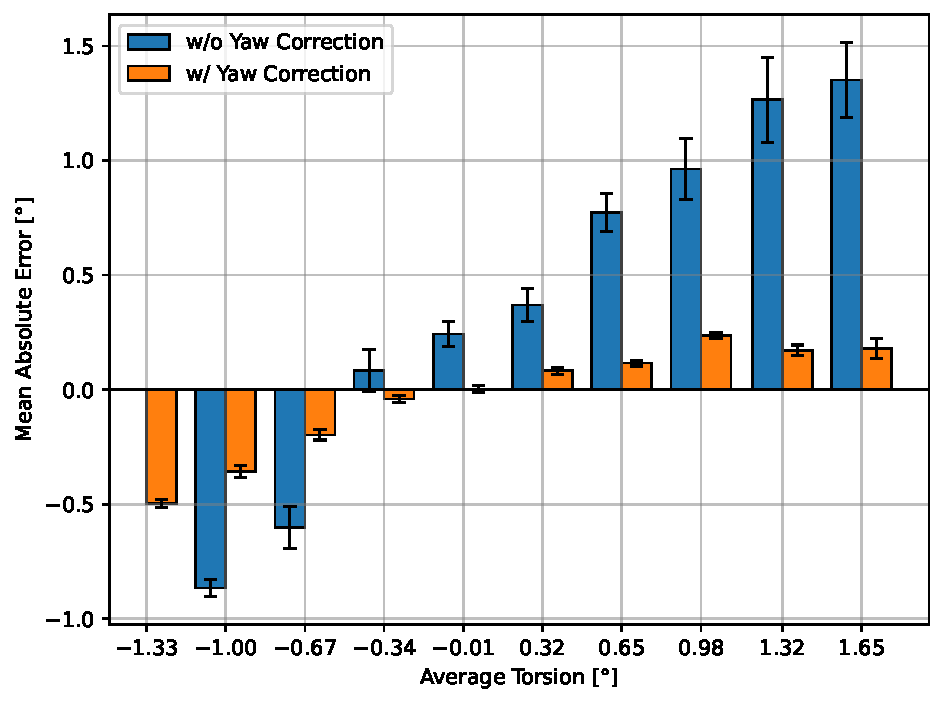
\includegraphics[width=0.6\linewidth]{graphics/yaw_error_bars_binned.pdf}
		\caption{Average error as a function of the average torsion grouped in 10 equally spaced and sized bins.}
		\label{fig:yaw_error_plot}
	\end{figure}
	
	\Cref{tab:yaw_error_sum} summarizes the error measurements for both the uncorrected and corrected average torsion signals.
	\begin{table}[h]
		\centering
		\begin{tabular}{cccc}
			\toprule
			Time Series & MAE [\unit{\degree}] & Max. Absolute Error [\unit{\degree}] & SEM (\qty{95}{\percent}) [\unit{\degree}] \\
			\midrule
			w/o Yaw Correction & 4.14 & 9.88 & 0.085 \\
			w/ Yaw Correction & 0.26 & 1.07 & 0.008 \\
			\bottomrule
		\end{tabular}
		\caption{Summary of error measurements for the corrected and uncorrected in-plane deformation signals.}
		\label{tab:yaw_error_sum}
	\end{table}
	
	
	
	\section{Blade Pitch Angle Correction}
	
	\subsection{Problem Statement}
	
	As previously explained, the second to last step in the currently employed DIC pipeline (see Appendix \ref{appendix:a}), embodied in the \textit{align\_coordinate\_system.py} script, relies on a series of linear transformations to eliminate
	the rigid body rotation of the wind turbine rotor. This process is then followed by exporting the location of a point across time for each of the identified AoIs on the blade, values which are then finally used to quantify their in-plane, out-of-plane and torsional deformation.
	
	The flow diagram shown in \cref{fig:new_ablauf} helps visualize the current sequence of transformations carried out on the \textit{.out} files within the script. As mentioned in the previous chapter, these alignment transformations are carried out individually for each recorded frame on the complete point cloud (i.e. all valid points on all three blades), virtually eliminating both the rotor rotation and the changes in wind turbine yaw throughout the measurement.
	
	Since the DIC measurements are carried out on a pitch-controlled turbine, each blade can also vary its pitch angle independently during operation. A byproduct of applying global transformations to all points is the inability to remove the effects of these individual pitch rotations out of the points on each blade before calculating their deformation values. This manifests itself as the presence of clearly blade pitch-dependent artifacts on the final deformation time-series. This effect is especially clear in the in-plane deformation values; a clear example of this can be seen in \cref{fig:problem_statement} using data from the \textit{Messung 24} measurement.
	\begin{figure}[h!]
		\centering
		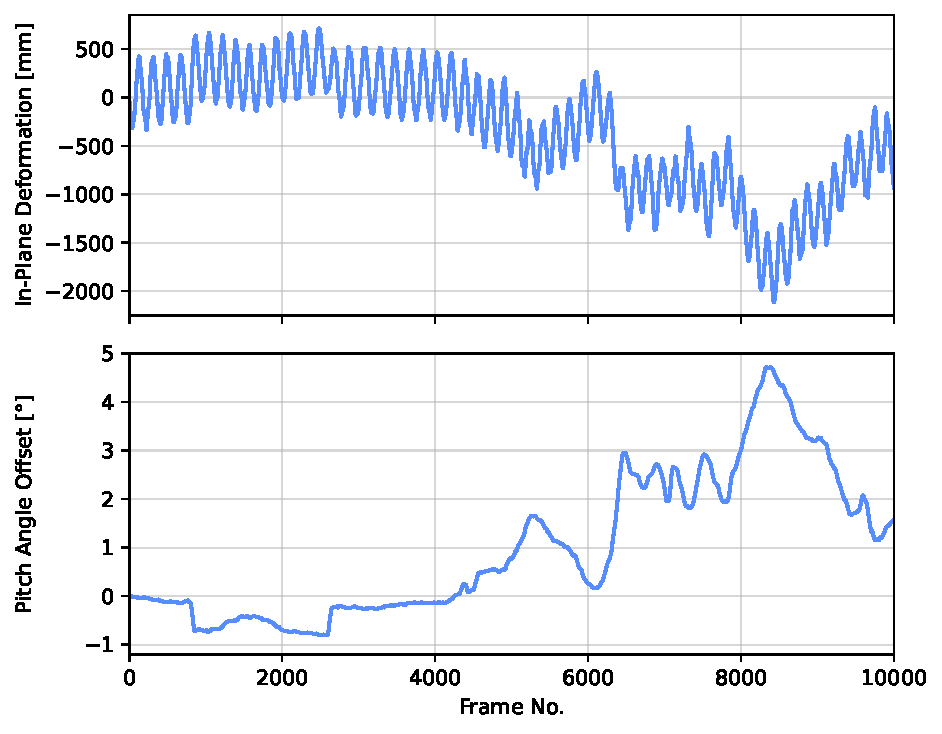
\includegraphics[width=0.6\linewidth]{graphics/problem_statement.pdf}
		\caption{In-plane deformation of blade A during the first 10,000 frames of the \textit{Messung 24} measurement plotted on top of the pitch angle offset.}
		\label{fig:problem_statement}
	\end{figure}
	
	
	
	\subsection{Correction Approach}
	Part of the dataset obtained from each field measurement contains a time series of the blade pitch angle value. In a nutshell, the correction process makes use of these values to virtually "un-pitch" all three blades individually in each frame. These new coordinate values are then stored as a new set of \textit{.out} files that are then used as a base for the rest of the transformations carried out in the script.
	
	It is assumed that all points in a given blade rotate about a fixed pitch axis throughout the measurement. The origin and orientation of this axis is approximated by fitting a cylinder to the innermost AoI of each blade; once all three pitch axes have been determined, the points corresponding to each blade are corrected using a sequence of linear transformations in the following order:
	\begin{enumerate}
		\item Bring the blade axis origin to the global origin.
		\item Rotate the blade points so that its pitch axis is aligned with the global z-axis.
		\item Rotate the blade points about the corresponding pitch angle offset relative to the first frame (i.e. $\Delta \theta_{i} = \theta_{i} - \theta_{0}$) in the negative direction to "unpitch" the blade.
		\item Apply the inverse rotation to bring the blade axis back to its original orientation.
		\item Apply the inverse offset to bring back the blade origin to its original location.
	\end{enumerate}
	
	Appendix \ref{app:pitch} helps visualize the complete correction process on a single blade (note that an exaggerated pitch value of \qty{45}{\degree} has been used there to aid in visualization). Once all three blades have been corrected for the current frame, a new \textit{.out} file for that frame is written and exported for use in the remaining of the script.
	
	
	\subsection{Results and Validation}
	A direct comparison of the resulting in-plane deformation values with and without correction can be seen in \cref{fig:mit}. When compared to the original signal, it is pretty evident how the orange line, corresponding to the corrected values, has been decoupled from the changes in the blade pitch, oscillating with a uniform amplitude about a consistent centre value throughout the measurement.
	\begin{figure}[h!]
		\centering
		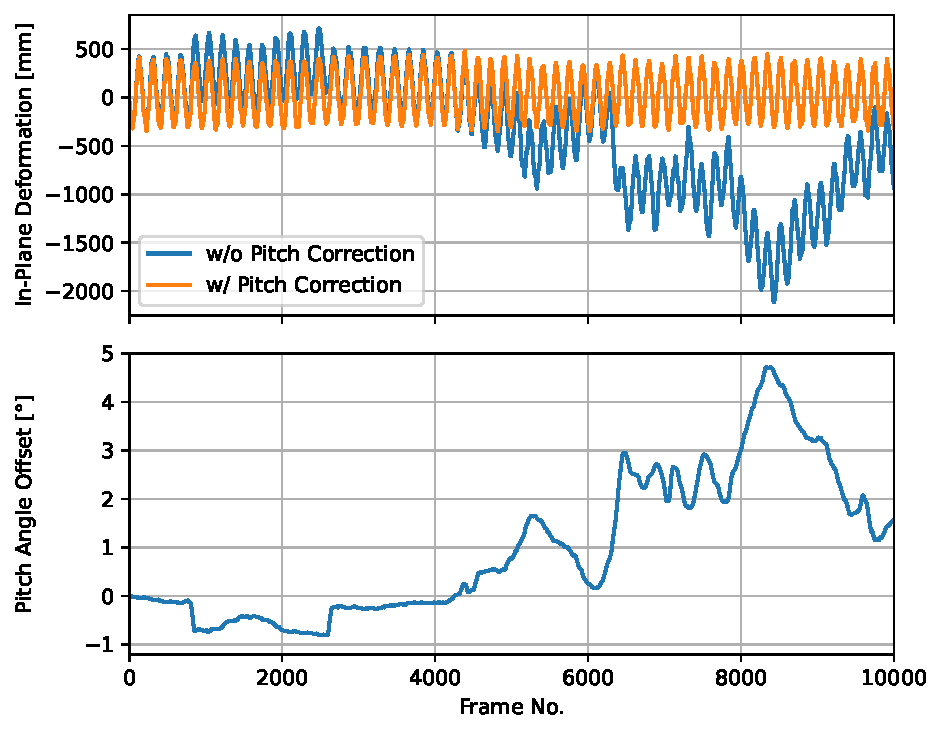
\includegraphics[width=0.6\linewidth]{graphics/results_messung24.pdf}
		\caption{In-plane deformation time-series for the third AoI in blade A with and without pitch correction.}
		\label{fig:mit}
	\end{figure}
	
	Similarly to the case of the yaw correction, it was not possible to quantitatively evaluate how good the corrected results were with respect to a known baseline given the lack of a known baseline and a synthetic dataset had to be generated to quantify the validity of the method.
	
	The Blender model used the pitch angle time series from measurement 24 as an input for pitch, the corrected in-plane and out-of-plane signals for its deformation. \Cref{fig:output} shows the resulting in-plane deformation signal for the three considered cases alongside the absolute error for both uncorrected and corrected signal. \Cref{tab:error_sum} summarizes the error measurements for both the uncorrected and corrected signals.
	\begin{figure}[h!]
		\centering
		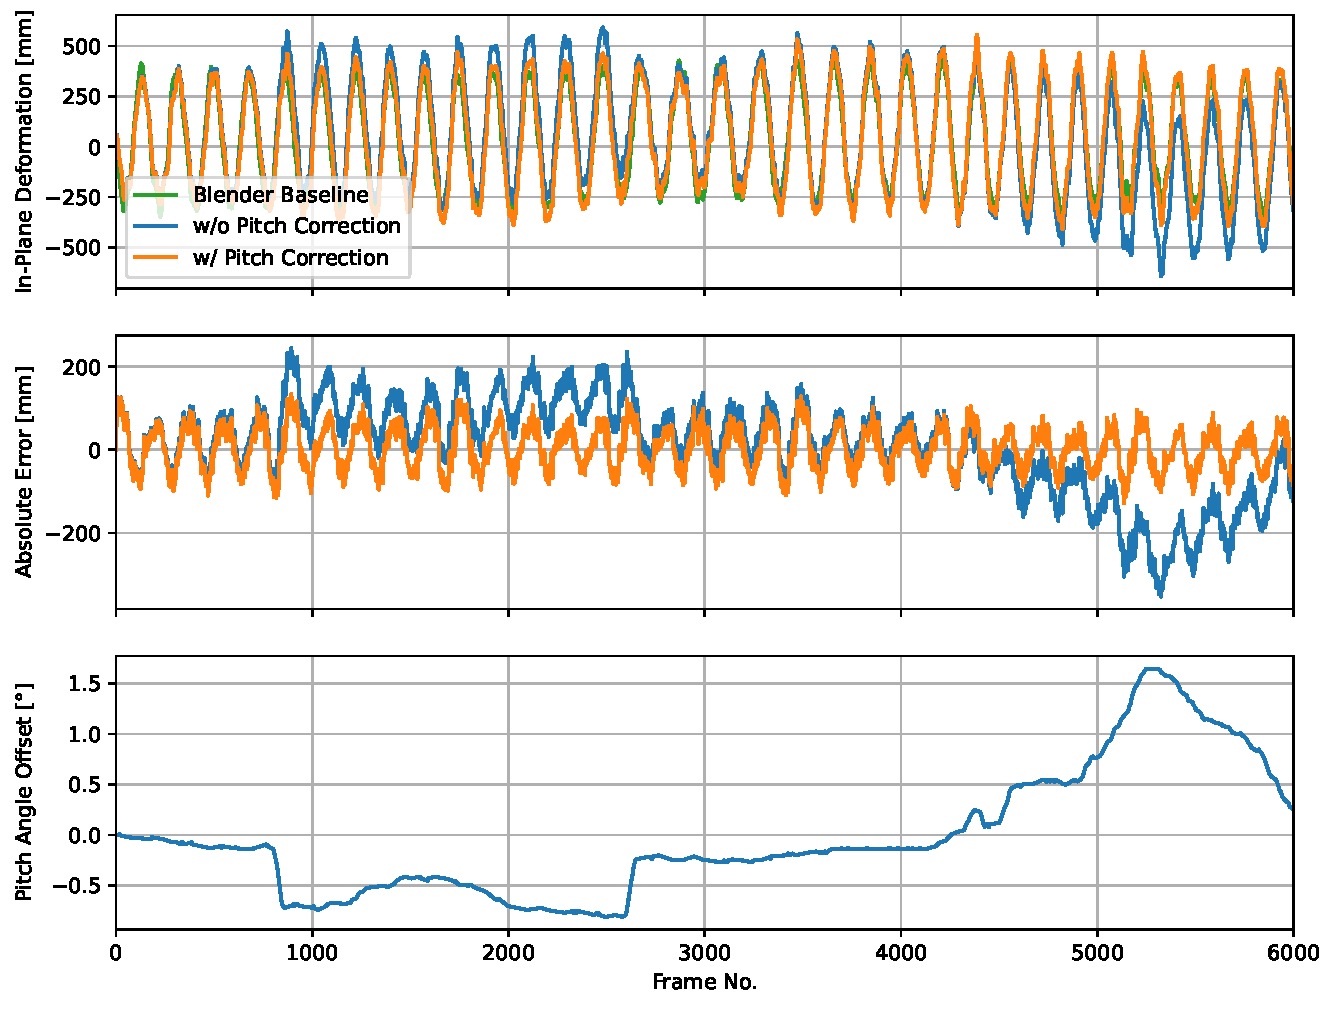
\includegraphics[width=0.6\linewidth]{graphics/results_blender.pdf}
		\caption{Baseline, corrected, and uncorrected in-plane deformation values for the synthetic measurement.}
		\label{fig:output}
	\end{figure}
	
	Analogous to the previous case, the absolute error as a function of the deflection is shown in \cref{fig:errorplot}. 
	\begin{figure}[h!]
		\centering
		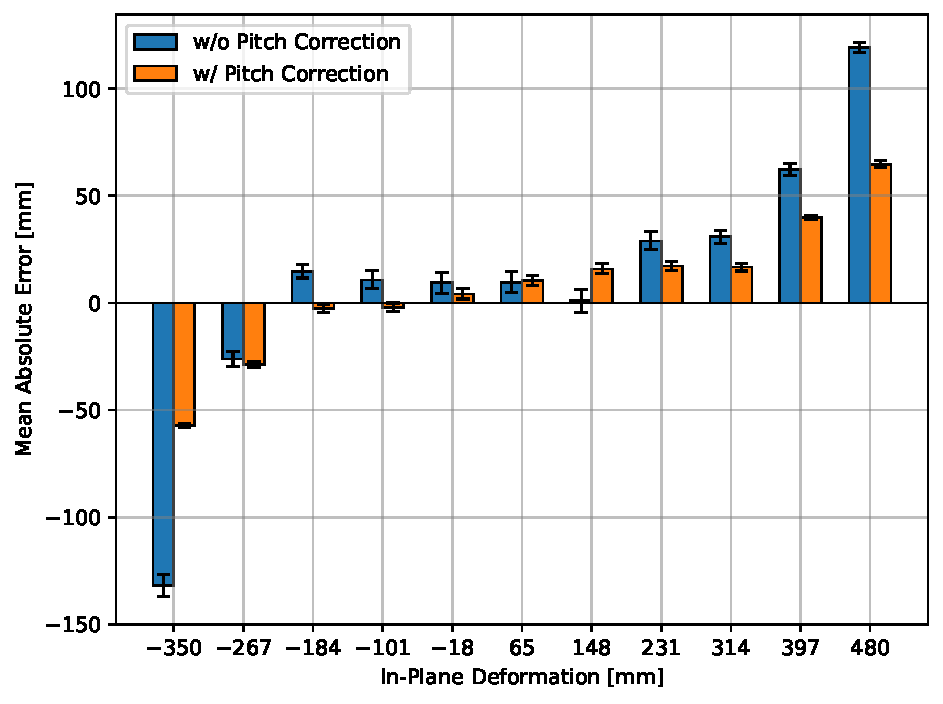
\includegraphics[width=0.6\linewidth]{graphics/error_bars_binned.pdf}
		\caption{Average error as a function of the in-plane deformation grouped in 10 equally spaced and sized bins.}
		\label{fig:errorplot}
	\end{figure}
	
	\begin{table}[h!]
		\centering
		\begin{tabular}{cccc}
			\toprule
			Time Series & MAE [\unit{\milli\meter}] & Max. Absolute Error [\unit{\milli\meter}] & SEM (\qty{95}{\percent}) [\unit{\milli\meter}]\\
			\midrule
			w/o Pitch Correction & \qty{91.2}{} & \qty{353.0}{} & \qty{3.29}{} \\
			w/ Pitch Correction & \qty{43.6}{} & \qty{127.4}{} & \qty{1.9}{} \\
			\bottomrule
		\end{tabular}
		\caption{Summary of error measurements for the corrected and uncorrected in-plane deformation signals.}
		\label{tab:error_sum}
	\end{table}
	
	\FloatBarrier
	\printbibliography[title=References]
	
	
	\clearpage
	\appendix
	\section{WEA DIC Pipeline}
	\label{appendix:a}
	
	\begin{figure}[htbp]
		\centering
		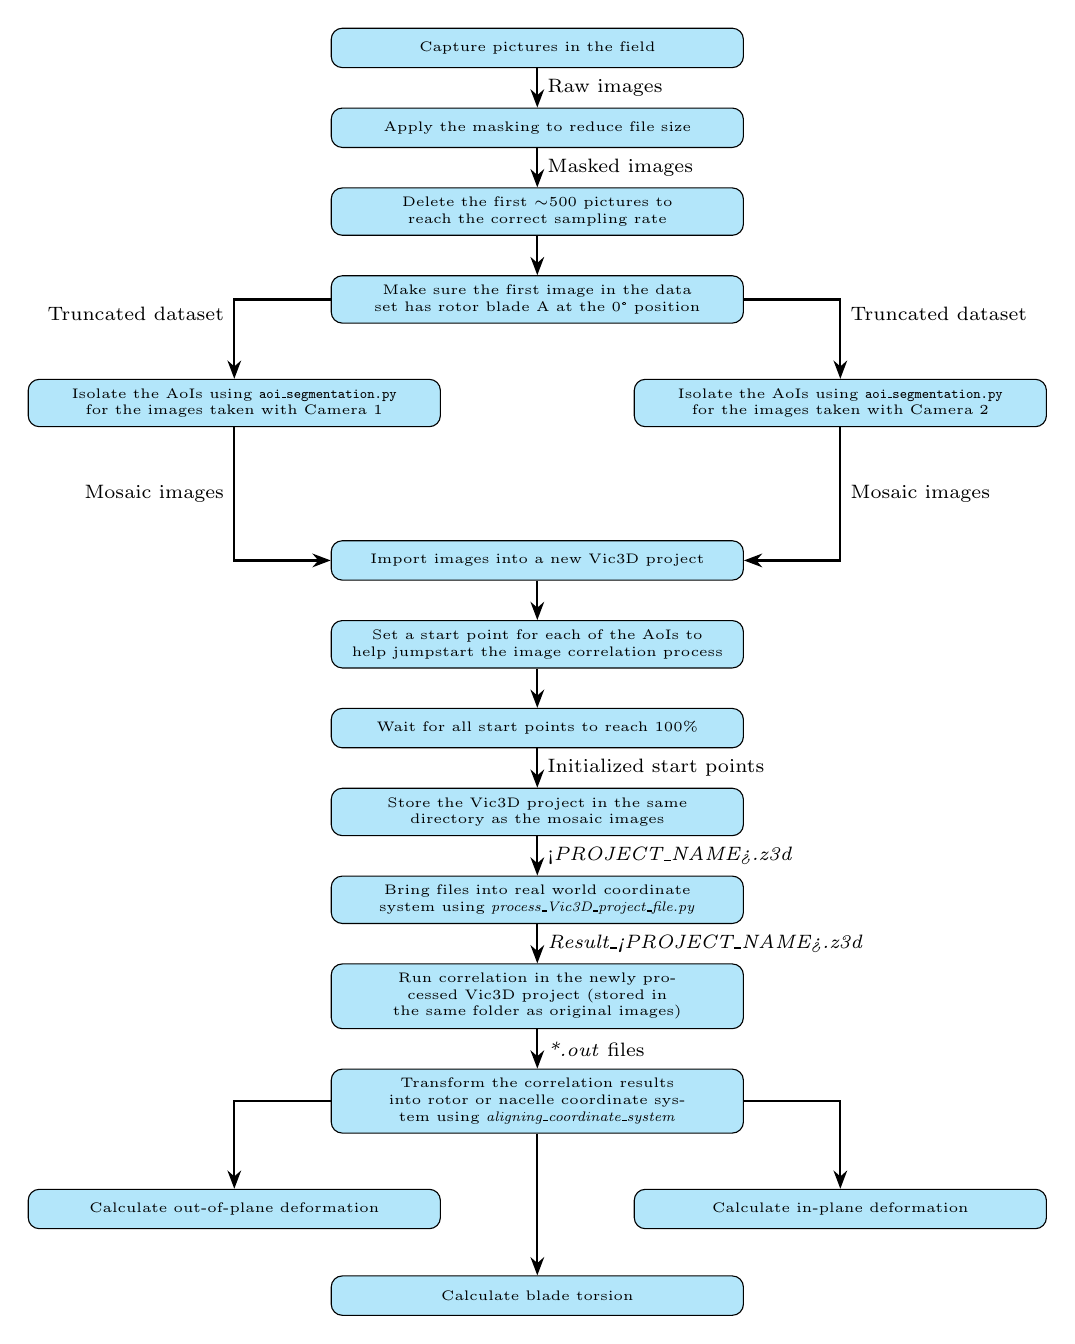
\begin{tikzpicture}[
			node distance=0.5cm and 0.5cm,
			mybox/.style={
				rectangle, 
				draw=black, 
				fill=cyan!30, 
				rounded corners, 
				text width=5cm, 
				align=center, 
				minimum height=0.5cm,
				font=\tiny
			},
			arrow/.style={-{Stealth}, thick}
			]
			
			% --- Main Vertical Flow (Top Part) ---
			\node (A) [mybox] {Capture pictures in the field};
			\node (B) [mybox, below=of A] {Apply the masking to reduce file size};
			\node (B1) [mybox, below=of B] {Delete the first $\sim$500 pictures to reach the correct sampling rate};
			\node (B2) [mybox, below=of B1] {Make sure the first image in the data set has rotor blade A at the 0\textdegree{} position};
			
			% --- Camera Split Branches ---
			\node (C) [mybox, below left=0.7cm and -1.4cm of B2] {Isolate the AoIs using \texttt{aoi\_segmentation.py} for the images taken with Camera 1};
			\node (D) [mybox, below right=0.7cm and -1.4cm of B2] {Isolate the AoIs using \texttt{aoi\_segmentation.py} for the images taken with Camera 2};
			
			% --- Merge to Vic3D ---
			\node (E) [mybox, below=1cm of B2, yshift=-1.75cm] {Import images into a new Vic3D project};
			\node (F) [mybox, below=of E] {Set a start point for each of the AoIs to help jumpstart the image correlation process};
			
			\node (G) [mybox, below=of F] {Wait for all start points to reach 100\%};
			
			\node (H) [mybox, below=of G] {Store the Vic3D project in the same directory as the mosaic images};
			
			\node (I) [mybox, below=of H] {Bring files into real world coordinate system using \textit{process\_Vic3D\_project\_file.py}};
			
			\node (J) [mybox, below=of I] {Run correlation in the newly processed Vic3D project (stored in the same folder as original images)};
			
			% --- Final Processing Branch ---
			\node (K) [mybox, below=of J] {Transform the correlation results into rotor or nacelle coordinate system using \textit{aligning\_coordinate\_system}};
			
			\node (L) [mybox, below left=0.7cm and -1.4cm of K] {Calculate out-of-plane deformation};
			\node (M) [mybox, below right=0.7cm and -1.4cm of K] {Calculate in-plane deformation};
			\node (N) [mybox, below=1cm of K, yshift=-0.8cm] {Calculate blade torsion};
			
			% --- Connecting Arrows ---
			\draw [arrow] (A) -- node[right, font=\scriptsize] {Raw images} (B);
			\draw [arrow] (B) -- node[right, font=\scriptsize] {Masked images} (B1);
			\draw [arrow] (B1) -- (B2);
			
			% Split to C and D
			\draw [arrow] (B2) -| node[above left, pos=0.7, font=\scriptsize] {Truncated dataset} (C);
			\draw [arrow] (B2) -| node[above right, pos=0.7, font=\scriptsize] {Truncated dataset} (D);
			
			% Into E
			\draw [arrow] (C) |- node[near start, left, font=\scriptsize] {Mosaic images} (E);
			\draw [arrow] (D) |- node[near start, right, font=\scriptsize] {Mosaic images} (E);
			
			% Downward flow
			\draw [arrow] (E) -- (F);
			\draw [arrow] (F) -- (G);
			\draw [arrow] (G) -- node[right, font=\scriptsize] {Initialized start points} (H);
			\draw [arrow] (H) -- node[right, font=\scriptsize]{<\textit{PROJECT\_NAME>.z3d}} (I); 
			\draw [arrow] (I) -- node[right, font=\scriptsize] {\textit{Result\_<PROJECT\_NAME>.z3d}} (J);
			
			% Post-J processing
			\draw [arrow] (J) -- node[right, font=\scriptsize] {\textit{*.out} files} (K);
			
			% Final split from K
			\draw [arrow] (K) -| (L);
			\draw [arrow] (K) -| (M);
			\draw [arrow] (K) -- (N);
			
		\end{tikzpicture}
		\caption{Complete processing pipeline for WEA DIC data acquisition and evaluation as described in \cite{winstroth2016leitfaden}.}
		\label{fig:wea_pipeline}
	\end{figure}
	
	\begin{landscape}
		\section{Pitch Correction of a Single Blade}
		\label{app:pitch}
		
		\vspace{1em} % Optional spacing between title and image
		\begin{center}
			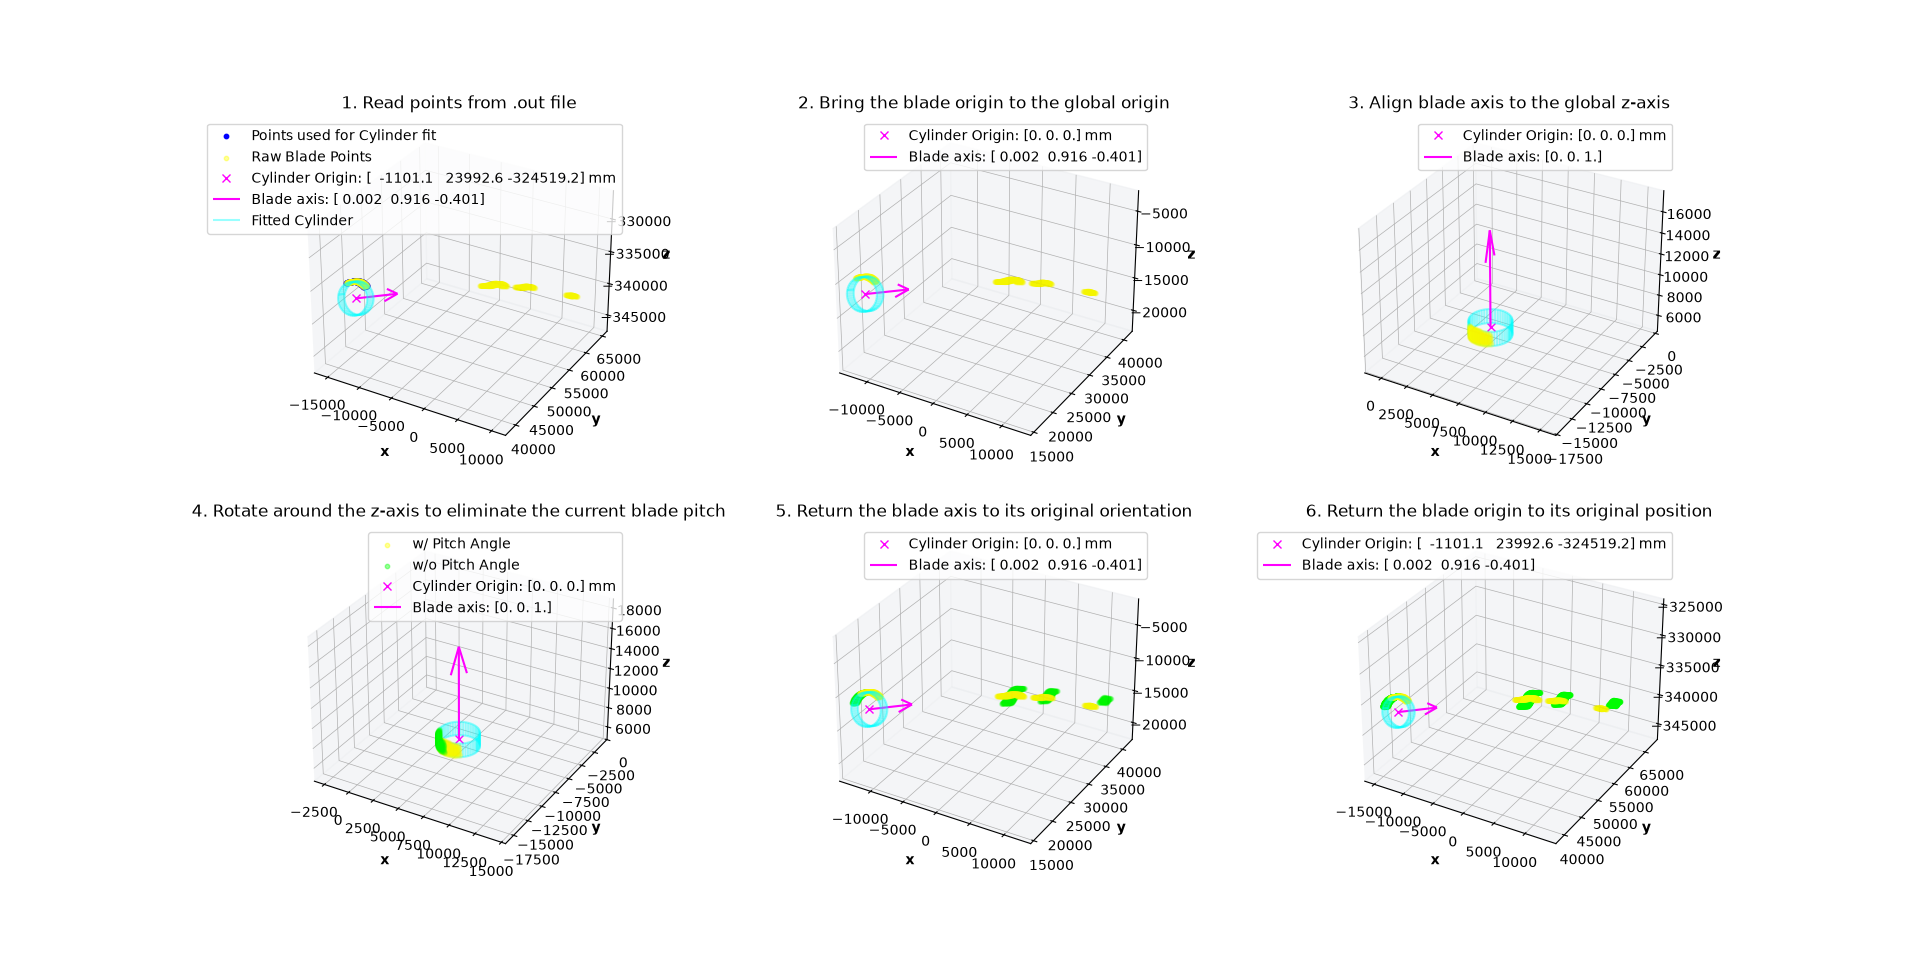
\includegraphics[width=\linewidth]{graphics/ansatz.png}
			\captionof{figure}{Pitch correction process exemplified with a single blade and an exaggerated \qty{45}{\degree} pitch value.}
			\label{fig:ansatz}
		\end{center}
	\end{landscape}
	
	
\end{document}